% METODOLOGIA------------------------------------------------------------------

\chapter{Implementação do Protótipo}
\label{chap:prototipo}

Este capitulo descreve a montagem do protótipo para testes. Será feita uma introdução do funcionamento geral, e suas principais características. Posteriormente será mostrado o funcionamento da base de testes da câmera, conexões entre os servo motores e os pinos GPIO, instalação e configuração do sistema operacional para o Raspberry Pi, e desenvolvimento do programa e controle dos servo motores, desenvolvimento do aplicativo Android, responsável por capturar dados dos sensores de posição e envio pela rede sem fio.

\section{Especificação do Projeto}
\label{sec:especificacao}

Apesar de ser composto por diversos módulos, o projeto pode ser dividido conceitualmente em duas partes, denominados por módulo de coleta de dados, ou celular Android, e módulo de controle de câmera, ou Raspberry Pi. O módulo de controle de câmera é responsável por receber os dados de posição através de uma conexão socket, converter o sistema de coordenadas, aplicar um filtro para evitar o acionamento desnecessário dos motores e acionar os servos, quando necessário. O módulo de coleta de dados é responsável por configurar os sensores de localização disponíveis no smartfone, aplicar os filtros necessários para minimizar ruídos na coleta de dados, encontrar o módulo de controle de câmeras através de uma busca na rede e enviar para ele, os dados das coordenadas através de uma conexão socket. \par

\begin{figure}[H]
	\centering
	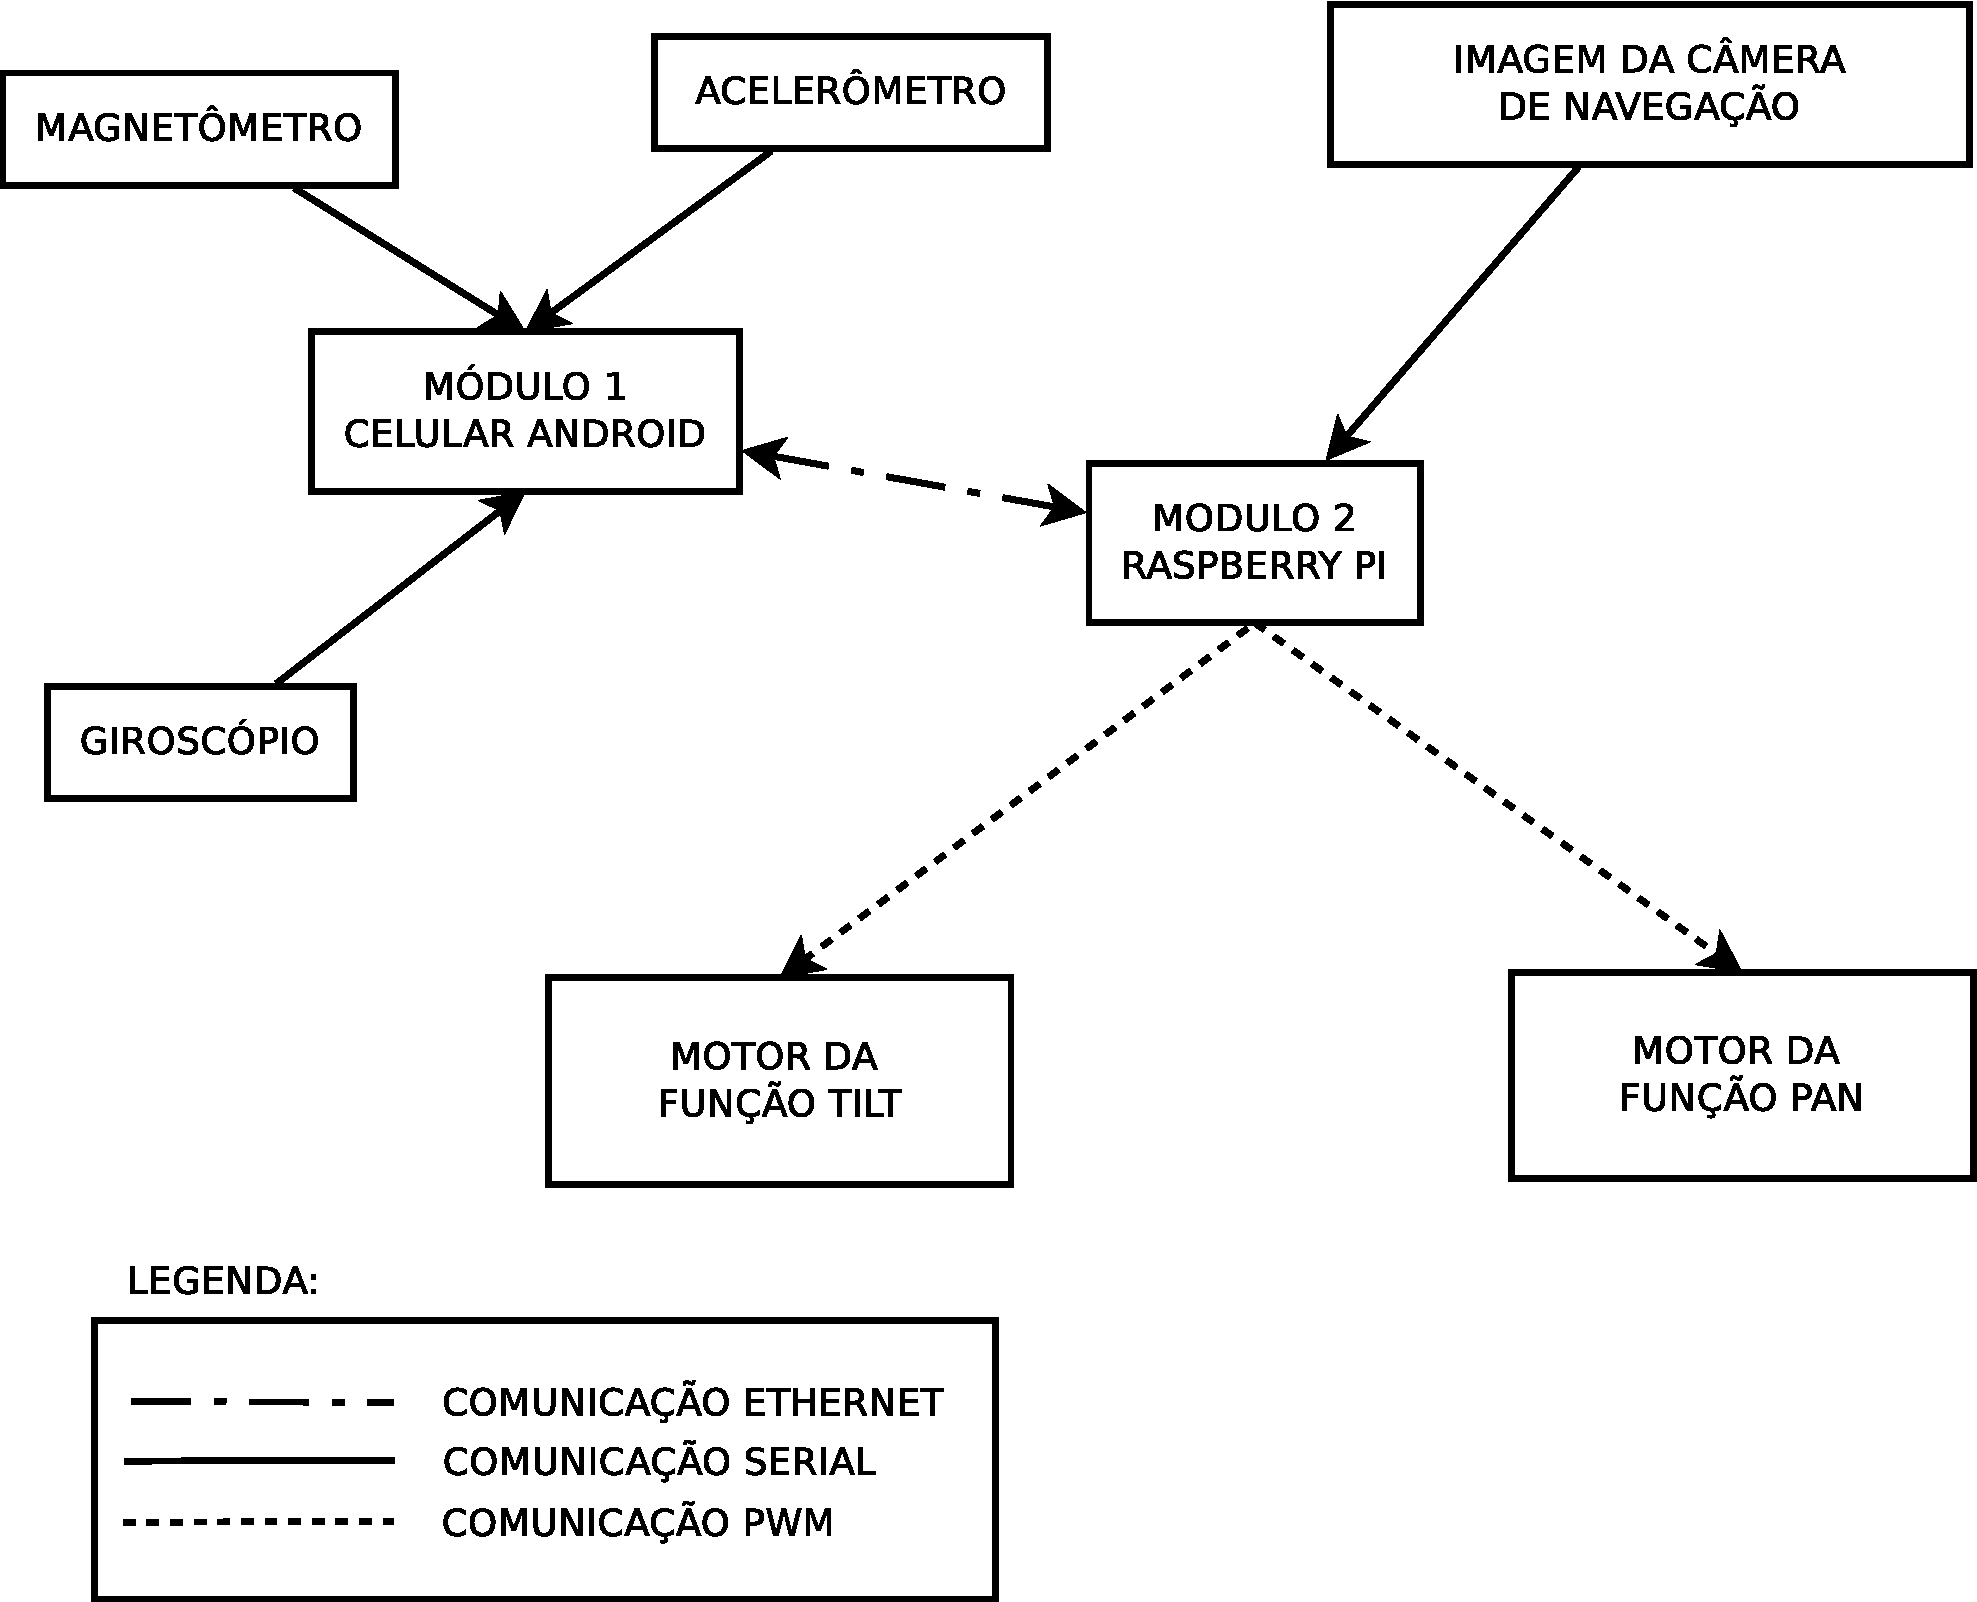
\includegraphics[width=0.7\textwidth]{figuras/diagrama-modulos-eps-converted-to.pdf}
	\caption{Diagrama de blocos da comunicação entre os módulos}
	\label{fig:diagrama_blocos}
\end{figure}

A \autoref{fig:diagrama_blocos} mostra como cada módulo se comunica com seus sensores, atuadores e entre sí. Os sensores estão embarcados no smartfone e não serão controlados separadamente. O sistema operacional Android fornece uma abstração para o hardware, e portanto não será necessário configurar os sensores manualmente. 

\subsection{Módulo de Controle de Câmeras}
\label{subsec:modconcam}

O módulo de controle de câmeras consiste em um SoC Raspberry Pi 1 modelo B, que possui um processador ARM de 700MHz, 512Mb de memória RAM, 26 pinos de proposito geral (GPIO), dua portas USB e uma porta Ethernet. Que tem as seguintes responsabilidades:

\begin{itemize}
	\item Responder requisições broadcast particular que identifica o módulo
	\item Receber dados de posição de sensores
	\item Filtrar os dados recebidos para evitar acionamento desnecessário dos motores
	\item Traduzir coordenadas dos sensores para coordenadas das câmeras
	\item Acionar dois motores servos de acordo coordenadas recebidas
\end{itemize}

\subsection{Módulo de Captura de Movimento}
\label{subsec:modcapmov}

O módulo de envio de coordenadas é um smartfone Android Motorola G6 com processador ARM Qualcomm Snapdragon 450 1,8 GHz Octa-Core, 3GB de memoria RAM, conectividade Wi-Fi, que possui os seguinte sensores: Acelerômetro, Magnetômetro, Giroscópio, Proximidade, Luz Ambiente e leitor de Impressão Digital. Que é responsável por:

\begin{itemize}
	\item Enviar requisição broadcast especial para detectar o módulo de controle de câmeras
	\item Conectar no módulo de controle de câmera
	\item Configurar sensores específicos para detecção de movimento
	\item Coletar dados dos sensores de movimento
	\item Aplicar filtro para evitar ruido na coleta dos dados de movimento
	\item Enviar coordenadas para o módulo de controle de câmera
\end{itemize}

\section{Montagem do Protótipo}
\label{sec:assemprototipo}

O protótipo foi construído usando uma fonte de alimentação de computador de mesa, padrão ATX, como fonte de alimentação e suporte para os outros componentes com exceção do smartfone Android.\par
Cola quente foi usada para fixar o Raspberry Pi, o corpo de montagem da câmera e motores servos (suporte articulado) e um ponto de acesso sem fio, que fornece a infra-estrutura de rede Wi-Fi para o projeto, à fonte e base. \par
O suporte dos motores servo e da câmera é uma estrutura moldada em plástico, observado na \autoref{fig:basedesmontada}, que precisa ser montada com parafusos e fixa os motores em sua posição de descanso (centro de curso), não sendo possível modificar está posição facilmente depois de montado, ilustrado na \autoref{fig:basemontada}.\par

\begin{figure}[H]
	\centering
	\begin{subfigure}{.5\textwidth}
		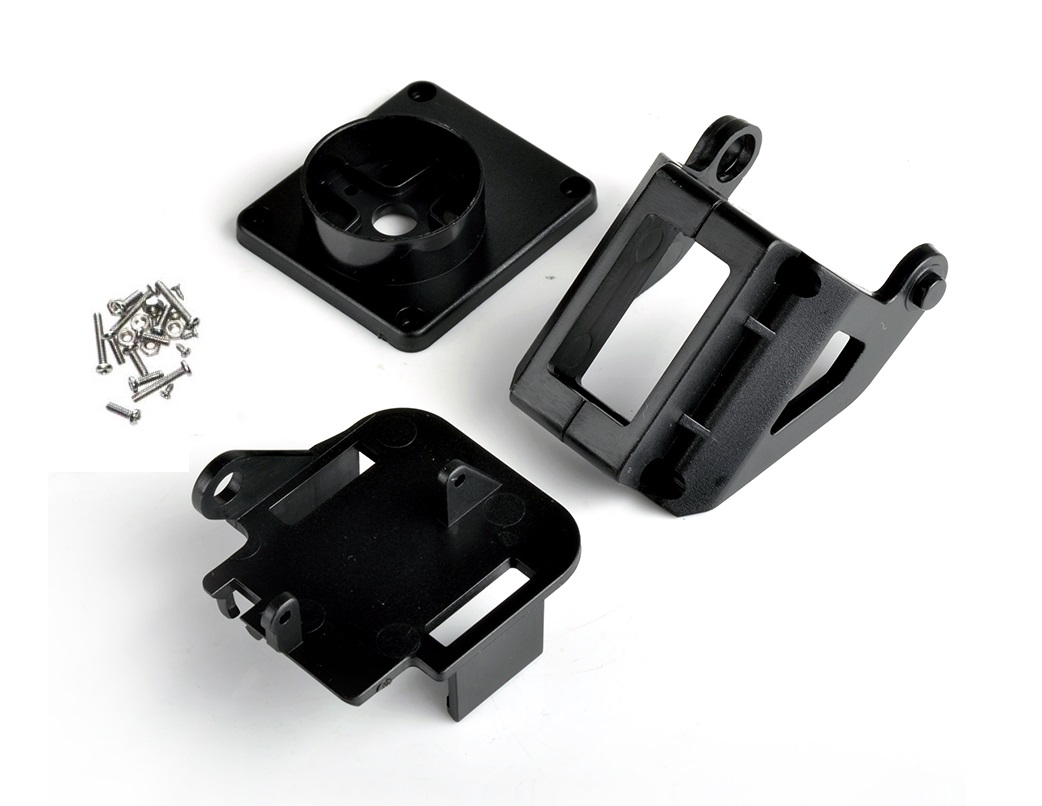
\includegraphics[width=0.95\textwidth]{figuras/base2.jpg}
		\caption{Componentes do suporte.}
		\label{fig:basedesmontada}
	\end{subfigure}%
	\begin{subfigure}{.5\textwidth}
		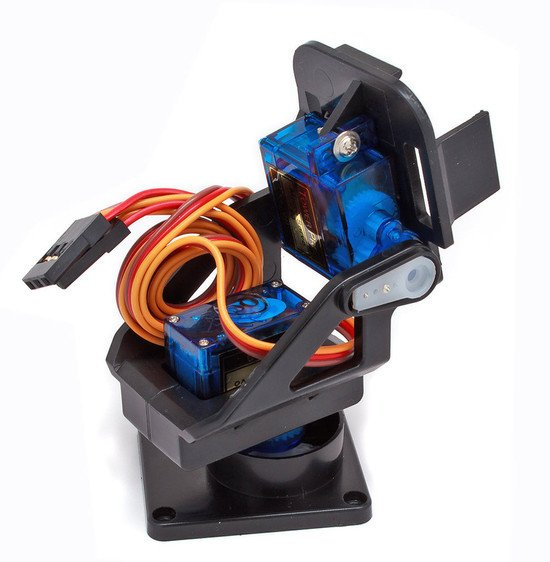
\includegraphics[width=0.75\textwidth]{figuras/base3.jpg}
		\caption{Montagem com motores.}
		\label{fig:basemontada}
	\end{subfigure}
	\caption{Base de suporta para motores e câmera.}
\end{figure}

Com a intensão de testar os motores, e preservar o Raspberry Pi (um dispositivo menos tolerante a falhas quando se trata de níveis de tensão nos pinos de propósito geral), foi desenvolvido um circuito gerador de PWM (drive PWM), onde era possível ajustar tanto a frequência do sinal quanto a largura dos pulsos, através de mudança de resistores e um potenciômetro. O propósito do circuito foi descobrir a posição central dos motores e verificar sua estabilidade enquanto se variava a frequência do sinal. O drive foi montado usando o circuito integrado NE555, um componente eletrônico bastante usado em aplicações que envolve temporização, geração de pulso e PWM. \par

Ativando individualmente os motores com o drive construído e com o auxilio de um osciloscópio, foi possível notar que os motores operam de forma estável com pulsos gerados numa frequência de 50Hz, e que é possível controlar a sua posição variando a largura do pulso entre valores próximos a 1ms, posição de angulo $180\degree$ (ângulo máximo), e valores próximos 2ms, posição de angulo $0\degree$ (ângulo mínimo), como ilustrado na \autoref{fig:pwmservo}. Foi possível observar também que existe uma correspondência linear entre a largura do pulso e a posição angular do eixo do motor, sendo assim, a posição de repouso ou centro, pode ser alcançada com uma largura de pulso próximo a 1,5 milissegundos. 

\begin{figure}[H]
	\centering
	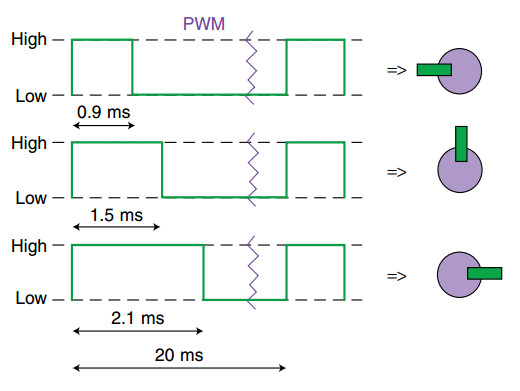
\includegraphics[width=0.7\textwidth]{figuras/pwm_servo.jpg}
	\caption{Posição do eixo do motor em função da largura de pulso PWM.}
	\fonte{\citeonline{pinckney2006pulse}}
	\label{fig:pwmservo}
\end{figure}

Para conectar os motores ao módulo de câmera (Raspberry Pi), foi necessário construir um circuito de acionamento dos motores, que consiste em dois transistores bipolares de junção (BJT), um para cada motor, configurados no modo emissor-comum, funcionando como um interruptor acionado pelo sinal PWM gerado pelos pinos GPIO do Raspberry Pi. A fonte do sinal PWM foi ligada ao terminal base do transistor através de um resistor de 1Kohm, com a função de limitar a corrente $I_b$ e a via de sinal do motor foi conectado ao terminal coletor do transistor e também a uma fonte de 5V através de um resistor de 10Kohm, responsável por limitar a corrente $I_c$, máxima quando o transistor está ativado, como ilustrado no circuito da .\par
Esse circuito foi construído numa mini \textit{breadboard} e tem o objetivo proteger o Raspberry Pi, evitando o consumo excessivo de corrente (mais que 15mA) ou uma possível corrente de retorno para um dos pinos GPIO numa eventual falha do circuito interno de controle dos motores. Como o circuito de proteção inverte o sinal PWM, foi necessário gerar um sinal invertido no módulo de controle de câmera, para que esse fosse invertido novamente pelo circuito de proteção e assim chegar como devido ao circuito de controle interno do motor.

\begin{figure}[H]
	\centering
	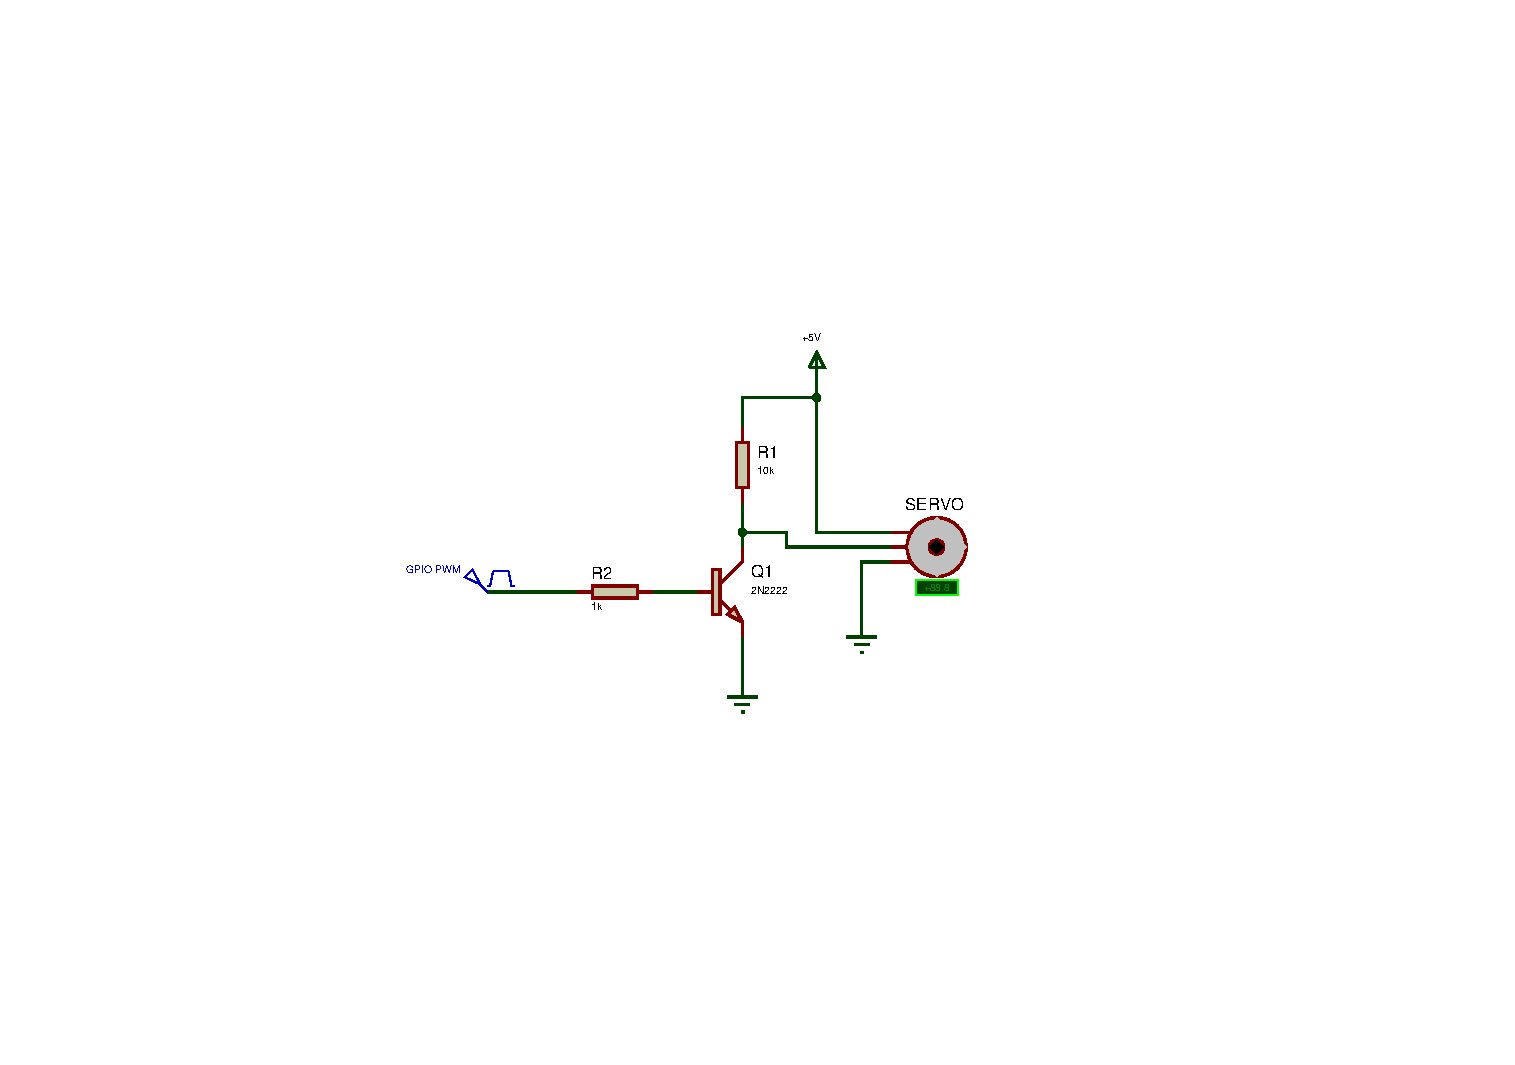
\includegraphics[trim={6.5cm 5cm 7.5cm 4cm},clip,width=0.7\textwidth]{figuras/circ_acionamento.pdf}
	\caption{Circuito de acionamento de motores.}
	\label{fig:circprotecao}
\end{figure}

\subsection{Montagem do Módulo de Controle de Câmera}
\label{subsec:assemmodconcam}

O módulo de controle de câmera na verdade controla os motores usados para movimentar uma câmera. 

- construção da classe server\\
- construção da classe servo\\
- construção da classe display\\
- construção da classe main\\

\subsection{Montagem do Módulo de Captura de Movimento}
\label{subsec:assemmodcapmov}

- instalação de pacotes necessarios para o desenvolvimento\\
- construção da classe Orientation\\
- construção da classe NetWorks\\
- construção da classe FullscreenActivity\\
